\documentclass{article}
\usepackage{graphicx}
\usepackage[utf8]{inputenc}
\usepackage{listings}
\usepackage{color}
\usepackage{xcolor}
\usepackage{textcomp}
\usepackage{amsmath}
\usepackage{mathabx}


\begin{document}

\title{Tarea spline cubico}
\author{Angel Caceres Licona}

\maketitle

\section{Use los nodos...}

Usando esos nodos obtenemos el siguiente polinomio:\\

$f(x) = -2.0000 * 10^{-63}* x^3 + 3.0000 * 10^{-63}* x^2 + 8.9258 * 10^{-1}* x -8.9258 * 10^{-1}$

Evaluado en $x=8.4$ obtenemos lo siguiente: 0.89258\\
El valor real es: 17.8771\\
Por lo que tenemos un valor absoluto de 16.98452, por lo que es una muy mala aproximación.\\
Tenemos la siguiente gráfica:\\
\begin{center}
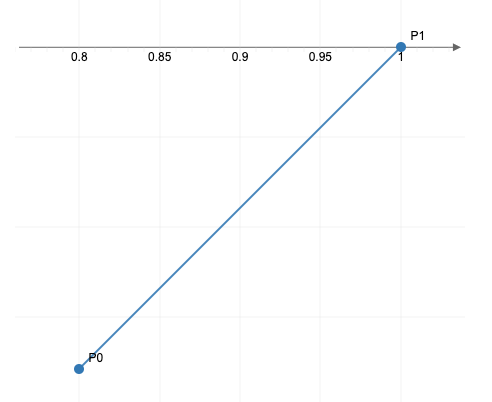
\includegraphics[scale=0.5]{grafica1.png}
\end{center}
\section{Ahora para la función $xcosx -2x^2 + 3x -1$}
Para esta función y los nodos dados obtenemos lo siguiente:\\
$f(x) = \begin{cases}-8.9957* x^3 + 2.6987* x^2 + 3.1852* x -9.5701 * 10^{-1}, & \text{si } x \in [0.1,0.2], \\
    -9.4662 * 10^{-1}* x^3 -2.1307* x^2 + 4.1511* x -1.0214, & \text{si } x \in (0.2,0.3], \\
    9.9423* x^3 -1.1931 * 10^{1}* x^2 + 7.0911* x -1.3154, & \text{si } x \in (0.3,0.4].\end{cases}$
\begin{center}
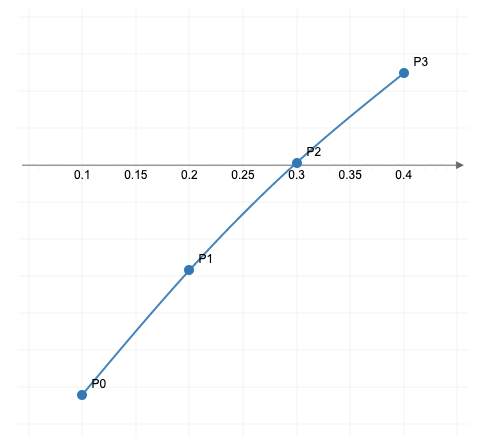
\includegraphics[scale=0.5]{grafica2.png}
\end{center}
El valor calculado es $f(0.25)=-0.13159$ y el valor real es $-0.132772$ y el error absoluto es: $0.264362$

\section{Calcule e integre el polinomio...}
Para esta función y los nodos dados obtenemos lo siguiente:\\
$f(x) = \begin{cases}-6.6274* x^3 + 8.3848 * 10^{-61}* x^2 -7.5736 * 10^{-1}* x + 1.0000, & \text{si } x \in [0,0.25], \\
    6.6274* x^3 -9.9411* x^2 + 1.7279* x + 7.9289 * 10^{-1}, & \text{si } x \in (0.25,0.5], \\
    6.6274* x^3 -9.9411* x^2 + 1.7279* x + 7.9289 * 10^{-1}, & \text{si } x \in (0.5,0.75], \\
    -6.6274* x^3 + 1.9882 * 10^{1}* x^2 -2.0640 * 10^{1}* x + 6.3848, & \text{si } x \in (0.75,1].\end{cases}$
\begin{center}
    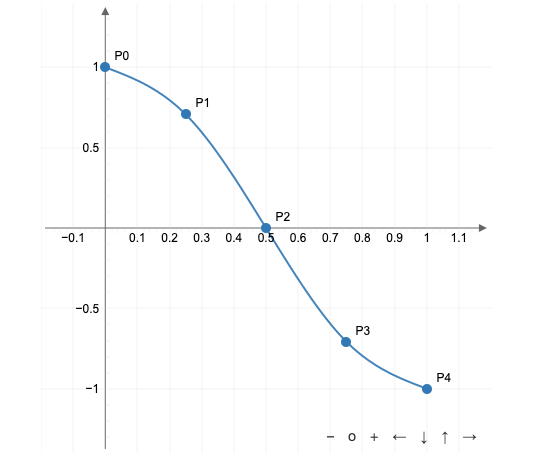
\includegraphics[scale=0.5]{grafica3.png}
\end{center}
El valor calculado de la integral es ${0.0947332}$ y el valor real es $0$ y el error absoluto es: $0.264362$ por lo que no da una buena aproximación.\\
Luego $f'(0.5) = -5.72791$ el valor real es: $-3.14159$\\
Y $f''(0.5) = {-19.8822}$ el valor real es: $-6.04339*10^{-16}$

\section{Demuestre que el polinomio de grado 3...}
Este polinomio cumple las 5 condiciones de spline cúbico pero no cumple la condición 6.a de spline natural.
\end{document}